\documentclass{standalone}
\usepackage{tikz}
\usetikzlibrary{patterns, positioning}


\begin{document}
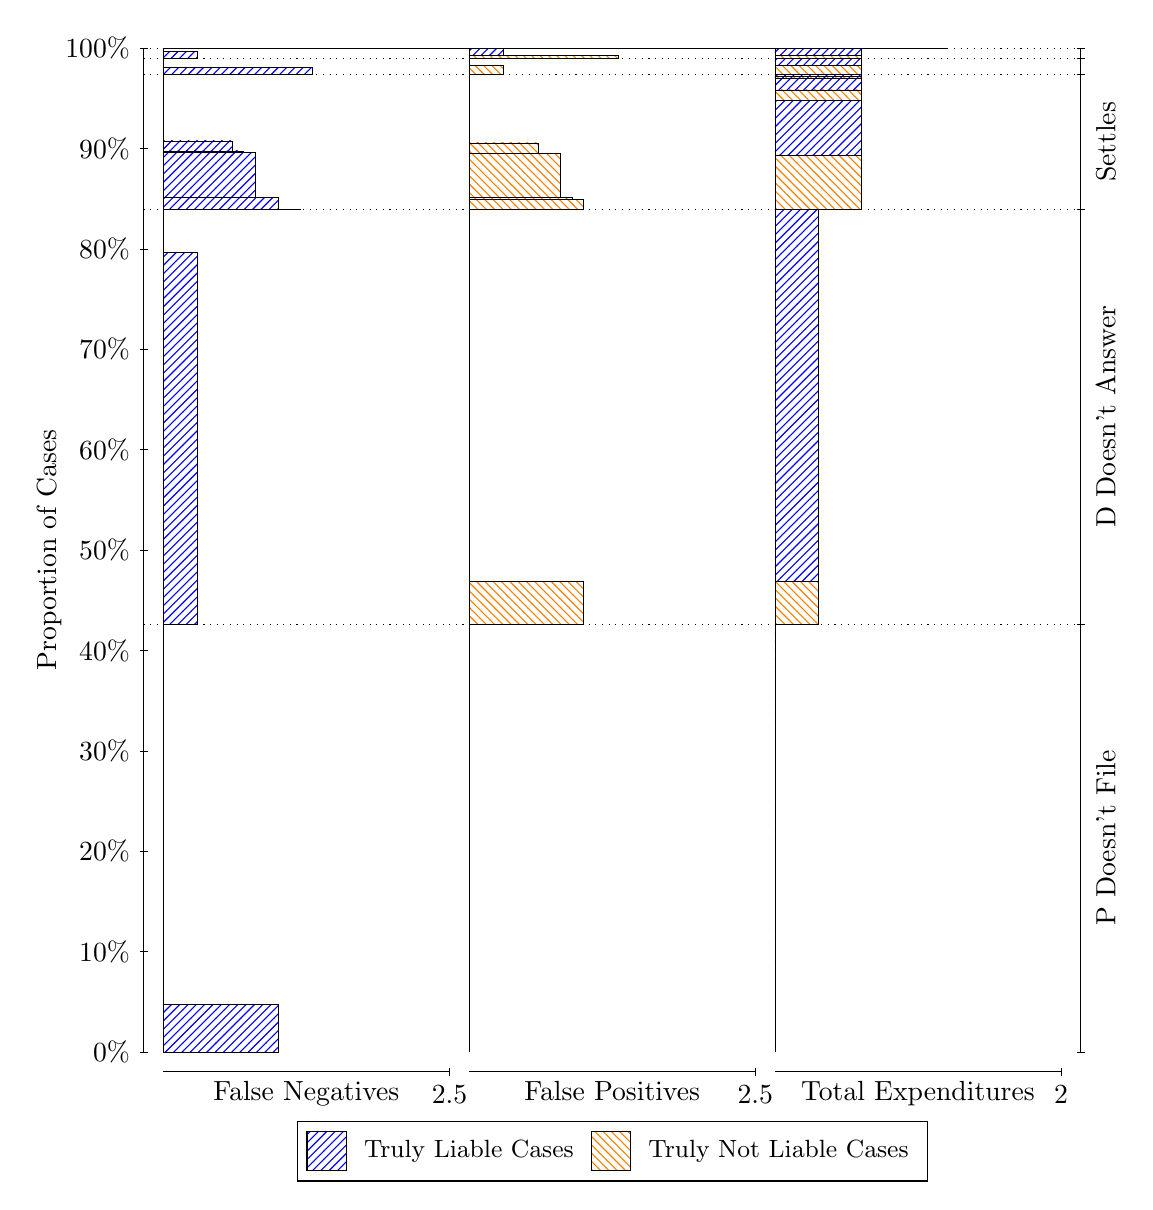
\begin{tikzpicture}
\draw[black, very thin] (1.5,1.75) -- (1.5,14.5);
\node[rotate=90, text=black, anchor=center] at (0.3, 8.125) {Proportion of Cases};
\draw[black, very thin] (1.45,1.75) -- (1.55,1.75);
\node[text=black, anchor=east] at (1.45, 1.75) {0\%};
\draw[black, very thin] (1.45,3.025) -- (1.55,3.025);
\node[text=black, anchor=east] at (1.45, 3.025) {10\%};
\draw[black, very thin] (1.45,4.3) -- (1.55,4.3);
\node[text=black, anchor=east] at (1.45, 4.3) {20\%};
\draw[black, very thin] (1.45,5.575) -- (1.55,5.575);
\node[text=black, anchor=east] at (1.45, 5.575) {30\%};
\draw[black, very thin] (1.45,6.85) -- (1.55,6.85);
\node[text=black, anchor=east] at (1.45, 6.85) {40\%};
\draw[black, very thin] (1.45,8.125) -- (1.55,8.125);
\node[text=black, anchor=east] at (1.45, 8.125) {50\%};
\draw[black, very thin] (1.45,9.4) -- (1.55,9.4);
\node[text=black, anchor=east] at (1.45, 9.4) {60\%};
\draw[black, very thin] (1.45,10.675) -- (1.55,10.675);
\node[text=black, anchor=east] at (1.45, 10.675) {70\%};
\draw[black, very thin] (1.45,11.95) -- (1.55,11.95);
\node[text=black, anchor=east] at (1.45, 11.95) {80\%};
\draw[black, very thin] (1.45,13.225) -- (1.55,13.225);
\node[text=black, anchor=east] at (1.45, 13.225) {90\%};
\draw[black, very thin] (1.45,14.5) -- (1.55,14.5);
\node[text=black, anchor=east] at (1.45, 14.5) {100\%};

\draw[black, very thin] (13.4,1.75) -- (13.4,14.5);
\draw[black, very thin] (13.35,1.75) -- (13.45,1.75);
\node[anchor=west] at (13.35, 1.75) {};
\draw[black, very thin] (13.35,7.1833) -- (13.45,7.1833);
\node[anchor=west] at (13.35, 7.1833) {};
\draw[black, very thin] (13.35,12.453) -- (13.45,12.453);
\node[anchor=west] at (13.35, 12.453) {};
\draw[black, very thin] (13.35,14.163) -- (13.45,14.163);
\node[anchor=west] at (13.35, 14.163) {};
\draw[black, very thin] (13.35,14.368) -- (13.45,14.368);
\node[anchor=west] at (13.35, 14.368) {};
\draw[black, very thin] (13.35,14.497) -- (13.45,14.497);
\node[anchor=west] at (13.35, 14.497) {};
\draw[black, very thin] (13.35,14.498) -- (13.45,14.498);
\node[anchor=west] at (13.35, 14.498) {};
\draw[black, very thin] (13.35,14.5) -- (13.45,14.5);
\node[anchor=west] at (13.35, 14.5) {};

\draw[black, very thin, pattern color=blue, pattern=north east lines] (1.75,1.75) rectangle (3.2033,2.357);
\draw[black, very thin, pattern color=orange, pattern=north west lines] (1.75,2.357) rectangle (1.75,7.1833);
\draw[black, very thin, pattern color=blue, pattern=north east lines] (1.75,7.1833) rectangle (2.186,11.908);
\draw[black, very thin, pattern color=orange, pattern=north west lines] (1.75,11.908) rectangle (1.75,12.453);
\draw[black, very thin, pattern color=blue, pattern=north east lines] (1.75,12.453) rectangle (3.494,12.454);
\draw[black, very thin, pattern color=blue, pattern=north east lines] (1.75,12.454) rectangle (3.3487,12.454);
\draw[black, very thin, pattern color=blue, pattern=north east lines] (1.75,12.454) rectangle (3.2033,12.607);
\draw[black, very thin, pattern color=blue, pattern=north east lines] (1.75,12.607) rectangle (3.058,12.608);
\draw[black, very thin, pattern color=blue, pattern=north east lines] (1.75,12.608) rectangle (2.9127,13.172);
\draw[black, very thin, pattern color=blue, pattern=north east lines] (1.75,13.172) rectangle (2.7673,13.194);
\draw[black, very thin, pattern color=blue, pattern=north east lines] (1.75,13.194) rectangle (2.622,13.321);
\draw[black, very thin, pattern color=orange, pattern=north west lines] (1.75,13.321) rectangle (1.75,14.163);
\draw[black, very thin, pattern color=blue, pattern=north east lines] (1.75,14.163) rectangle (3.6393,14.25);
\draw[black, very thin, pattern color=orange, pattern=north west lines] (1.75,14.25) rectangle (1.75,14.368);
\draw[black, very thin, pattern color=blue, pattern=north east lines] (1.75,14.368) rectangle (2.186,14.454);
\draw[black, very thin, pattern color=orange, pattern=north west lines] (1.75,14.454) rectangle (1.75,14.497);
\draw[black, very thin, pattern color=blue, pattern=north east lines] (1.75,14.497) rectangle (5.8193,14.497);
\draw[black, very thin, pattern color=orange, pattern=north west lines] (1.75,14.497) rectangle (1.75,14.498);
\draw[black, very thin, pattern color=orange, pattern=north west lines] (1.75,14.498) rectangle (1.75,14.498);
\draw[black, very thin, pattern color=blue, pattern=north east lines] (1.75,14.498) rectangle (1.75,14.5);
\draw[black, very thin, pattern color=orange, pattern=north west lines] (5.6333,1.75) rectangle (5.6333,6.5762);
\draw[black, very thin, pattern color=blue, pattern=north east lines] (5.6333,6.5762) rectangle (5.6333,7.1833);
\draw[black, very thin, pattern color=orange, pattern=north west lines] (5.6333,7.1833) rectangle (7.0867,7.7284);
\draw[black, very thin, pattern color=blue, pattern=north east lines] (5.6333,7.7284) rectangle (5.6333,12.453);
\draw[black, very thin, pattern color=orange, pattern=north west lines] (5.6333,12.453) rectangle (7.0867,12.58);
\draw[black, very thin, pattern color=orange, pattern=north west lines] (5.6333,12.58) rectangle (6.9413,12.6);
\draw[black, very thin, pattern color=orange, pattern=north west lines] (5.6333,12.6) rectangle (6.796,13.163);
\draw[black, very thin, pattern color=orange, pattern=north west lines] (5.6333,13.163) rectangle (6.6507,13.163);
\draw[black, very thin, pattern color=orange, pattern=north west lines] (5.6333,13.163) rectangle (6.5053,13.295);
\draw[black, very thin, pattern color=orange, pattern=north west lines] (5.6333,13.295) rectangle (6.36,13.295);
\draw[black, very thin, pattern color=orange, pattern=north west lines] (5.6333,13.295) rectangle (6.2147,13.296);
\draw[black, very thin, pattern color=blue, pattern=north east lines] (5.6333,13.296) rectangle (5.6333,14.163);
\draw[black, very thin, pattern color=orange, pattern=north west lines] (5.6333,14.163) rectangle (6.0693,14.281);
\draw[black, very thin, pattern color=blue, pattern=north east lines] (5.6333,14.281) rectangle (5.6333,14.368);
\draw[black, very thin, pattern color=orange, pattern=north west lines] (5.6333,14.368) rectangle (7.5227,14.41);
\draw[black, very thin, pattern color=blue, pattern=north east lines] (5.6333,14.41) rectangle (6.0693,14.497);
\draw[black, very thin, pattern color=orange, pattern=north west lines] (5.6333,14.497) rectangle (5.6333,14.497);
\draw[black, very thin, pattern color=blue, pattern=north east lines] (5.6333,14.497) rectangle (5.6333,14.498);
\draw[black, very thin, pattern color=orange, pattern=north west lines] (5.6333,14.498) rectangle (9.7027,14.498);
\draw[black, very thin, pattern color=blue, pattern=north east lines] (5.6333,14.498) rectangle (8.2493,14.5);
\draw[black, very thin, pattern color=orange, pattern=north west lines] (9.5167,1.75) rectangle (9.5167,6.5762);
\draw[black, very thin, pattern color=blue, pattern=north east lines] (9.5167,6.5762) rectangle (9.5167,7.1833);
\draw[black, very thin, pattern color=orange, pattern=north west lines] (9.5167,7.1833) rectangle (10.062,7.7284);
\draw[black, very thin, pattern color=blue, pattern=north east lines] (9.5167,7.7284) rectangle (10.062,12.453);
\draw[black, very thin, pattern color=orange, pattern=north west lines] (9.5167,12.453) rectangle (10.607,13.143);
\draw[black, very thin, pattern color=blue, pattern=north east lines] (9.5167,13.143) rectangle (10.607,13.835);
\draw[black, very thin, pattern color=orange, pattern=north west lines] (9.5167,13.835) rectangle (10.607,13.967);
\draw[black, very thin, pattern color=blue, pattern=north east lines] (9.5167,13.967) rectangle (10.607,14.122);
\draw[black, very thin, pattern color=orange, pattern=north west lines] (9.5167,14.122) rectangle (10.607,14.142);
\draw[black, very thin, pattern color=blue, pattern=north east lines] (9.5167,14.142) rectangle (10.607,14.163);
\draw[black, very thin, pattern color=orange, pattern=north west lines] (9.5167,14.163) rectangle (10.607,14.281);
\draw[black, very thin, pattern color=blue, pattern=north east lines] (9.5167,14.281) rectangle (10.607,14.368);
\draw[black, very thin, pattern color=orange, pattern=north west lines] (9.5167,14.368) rectangle (10.607,14.41);
\draw[black, very thin, pattern color=blue, pattern=north east lines] (9.5167,14.41) rectangle (10.607,14.497);
\draw[black, very thin, pattern color=orange, pattern=north west lines] (9.5167,14.497) rectangle (11.697,14.497);
\draw[black, very thin, pattern color=blue, pattern=north east lines] (9.5167,14.497) rectangle (11.697,14.498);
\draw[black, very thin, pattern color=orange, pattern=north west lines] (9.5167,14.498) rectangle (11.697,14.498);
\draw[black, very thin, pattern color=blue, pattern=north east lines] (9.5167,14.498) rectangle (11.697,14.5);
\draw[black, dotted] (1.5,7.1833) -- (13.4,7.1833);
\draw[black, dotted] (1.5,12.453) -- (13.4,12.453);
\draw[black, dotted] (1.5,14.163) -- (13.4,14.163);
\draw[black, dotted] (1.5,14.368) -- (13.4,14.368);
\draw[black, dotted] (1.5,14.497) -- (13.4,14.497);
\draw[black, dotted] (1.5,14.498) -- (13.4,14.498);
\draw[black, very thin] (1.75,1.5) -- (5.3833,1.5);
\node[text=black, anchor=north] at (3.5667, 1.5) {False Negatives};
\draw[black, very thin] (5.3833,1.45) -- (5.3833,1.55);
\node[text=black, anchor=north] at (5.3833, 1.45) {2.5};

\draw[black, very thin] (5.6333,1.5) -- (9.2667,1.5);
\node[text=black, anchor=north] at (7.45, 1.5) {False Positives};
\draw[black, very thin] (9.2667,1.45) -- (9.2667,1.55);
\node[text=black, anchor=north] at (9.2667, 1.45) {2.5};

\draw[black, very thin] (9.5167,1.5) -- (13.15,1.5);
\node[text=black, anchor=north] at (11.333, 1.5) {Total Expenditures};
\draw[black, very thin] (13.15,1.45) -- (13.15,1.55);
\node[text=black, anchor=north] at (13.15, 1.45) {2};

\node[text=black, centered, rotate=90] at (13.72, 4.4666) {P Doesn't File};
\node[text=black, centered, rotate=90] at (13.72, 9.8182) {D Doesn't Answer};
\node[text=black, centered, rotate=90] at (13.72, 13.308) {Settles};





\draw (7.449999999999999,1.5) node[draw=none] (baseCoordinate) {};
\begin{scope}[align=center]
        \matrix[scale=0.5, draw=black, below=0.5cm of baseCoordinate, nodes={draw}, column sep=0.1cm]{
            \node[rectangle, draw, minimum width=0.5cm, minimum height=0.5cm, pattern color=blue, pattern=north east lines] {}; &
            \node[draw=none, font=\small, text=black] (B) {Truly Liable Cases}; &
            \node[rectangle, draw, minimum width=0.5cm, minimum height=0.5cm, pattern color=orange, pattern=north west lines] {}; &
            \node[draw=none, font=\small, text=black] (B) {Truly Not Liable Cases}; \\
            };
\end{scope}

\end{tikzpicture}
\end{document}